\documentclass[a4paper]{article}
\usepackage[utf8]{inputenc}
\usepackage[T1]{fontenc}
\usepackage{graphicx}
\usepackage{hyperref}

\begin{document}

\noindent \textbf{Title}

\medskip

\noindent Nilearn: Machine learning and statistics for fMRI in Python

\bigskip

\noindent \textbf{Authors}

\medskip

\noindent Nicolas Gensollen,  Thomas Bazeille, Kshitij Chawla, Jerome-Alexis Chevalier, Kamalaker Dadi, Jérôme Dockès, Elizabeth DuPre, Daniel Gomez, Chris Gorgolewski, Alexandre Gramfort, Julia M Huntenburg, Eric Larson, Robert Luke, Chris Markiewicz, Binh Nguyen, Ana Luísa Pinho, Sylvain Takerkart, Bertrand Thirion, Alexis Thual, Taylor Tsalo, Gaël Varoquaux, Hao-Ting Wang

\bigskip

\noindent \textbf{Introduction}

\medskip

\noindent Efficient and reproducible science depends on a strong software ecosystem \cite{Poldrack2019}. We present here Nilearn, a Python package empowering the neuroimaging community by enabling fast and easy statistical learning on fMRI data: \url{https://nilearn.github.io}. It has been under continuous development for close to 10 years and just reached its 0.7 release. It is now part of the neuroimaging tools ecosystem with approximately 700 stars, 400 forks, and 135 contributors on GitHub, as well as more than 200 discussions on the forum Neurostars.

\medskip

\noindent Nilearn provides efficient and reliable implementations of machine learning methods tailored to the needs of the neuroimaging community. It builds upon a Python "data science ecosystem" of packages such as numpy \cite{VanDerWalt2011}, scipy \cite{Oliphant2007}, scikit-learn \cite{Pedregosa2011}, and pandas \cite{McKinney2010}, that are extensively used, tested and optimized by a large scientific and industrial community. This makes it easy to use for a broad spectrum of researchers who are familiar with the Python ecosystem. Specifically, Nilearn provides methods  for decoding functional connectivity analysis, and statistical parametric mapping. It also includes datasets for teaching, and interactive visualization of brain images and connectomes.

\bigskip

\noindent \textbf{Methods}

\medskip

\noindent Nilearn is a community-led open-source project, developed and used by researchers in neuroimaging and machine-learning. It strives to be easy to use with simple code and focuses only on reliable and well-established methods. User guides provide an introduction to machine learning and statistics for fMRI with examples showcasing all functionalities. Tutorials and coding sprints are also organized regularly to engage the neuroimaging community.

\medskip

\noindent Nilearn uses industry-standard methods for software development: source code is version controlled, functions are covered by unit tests that are run in a Continuous Integration framework, and several reviewers check every contribution. These best practices allow to incorporate contributions from around the world while preserving the quality and reliability of the code.

\bigskip

\noindent \textbf{Results}

\medskip

\noindent Nilearn is widely used and covers many of the analysis needs for neuroimaging:

\begin{itemize}
	\item Manipulation of brain images and basic signal processing;
	\item Supervised learning and decoding;
	\item Functional connectivity and decomposition methods;
	\item Plotting;
	\item Projection of volumetric data to surfaces;
	\item General Linear Model-based analysis and statistical testing;
	\item Model selection and validation, parallelism, and caching.
\end{itemize}

\noindent In its 0.7 release, Nilearn includes in a new glm module with all the functionalities of its previous sister’s project Nistats. This enables fitting mass univariate linear models in a consistent pipeline with simpler dependencies.

\medskip

\noindent A new Decoder object was also added to ease classification and regression tasks in a decoding pipeline. It implements a model selection scheme that averages the best models within a cross validation loop. These objects are tailored for usability and provide for example a direct interface with Nifti files on disk. In addition, the decoder objects pipeline have been extended with one fast clustering step at the beginning (yielding an implicit spatial regularization) and aggregates a high number of estimators trained on various splits of the training set. This returns a state-of-the-art decoding pipeline at a low computational cost (see fig. \ref{fig:figure_1}).

\medskip

\noindent Nilearn is also extensively used for its plotting capabilities (see fig. \ref{fig:figure_2}). New plotting functions have been added and enable, for example, plotting contours of regions of interest on surfaces, visualizing events file, or generating carpet plots for visualizing global patterns in 4D functional data over time.

\bigskip

\noindent \textbf{Conclusion}

\medskip

\noindent By following industry-standard methods and making analysis pipelines documented, version controlled, peer-reviewed, and shared, Nilearn targets the reproducibility crisis of neuroimaging by enabling researchers to produce pipelines that are intelligible, reproducible, and that can be extended to novel datasets.

\newpage


\begin{figure}[htp]
	\centering
	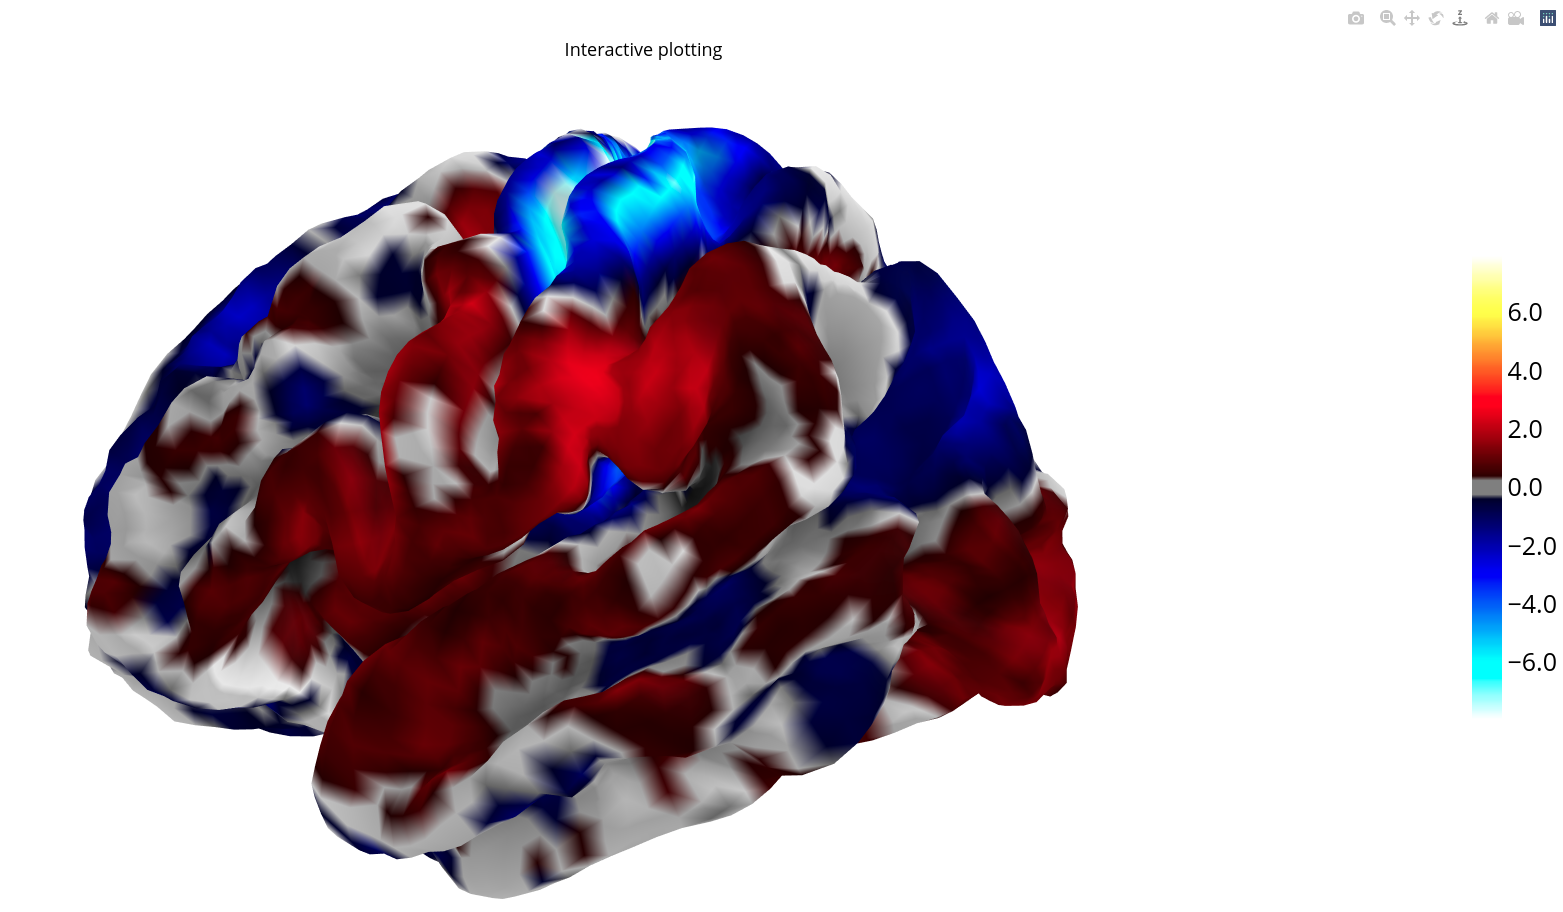
\includegraphics[scale=.8]{./figure_1}
	\caption{Example of loading data, fitting a decoder, and plotting the resulting statistical map in a few lines of Python code.}
	\label{fig:figure_1}
\end{figure}

\begin{figure}[hbp]
	\centering
	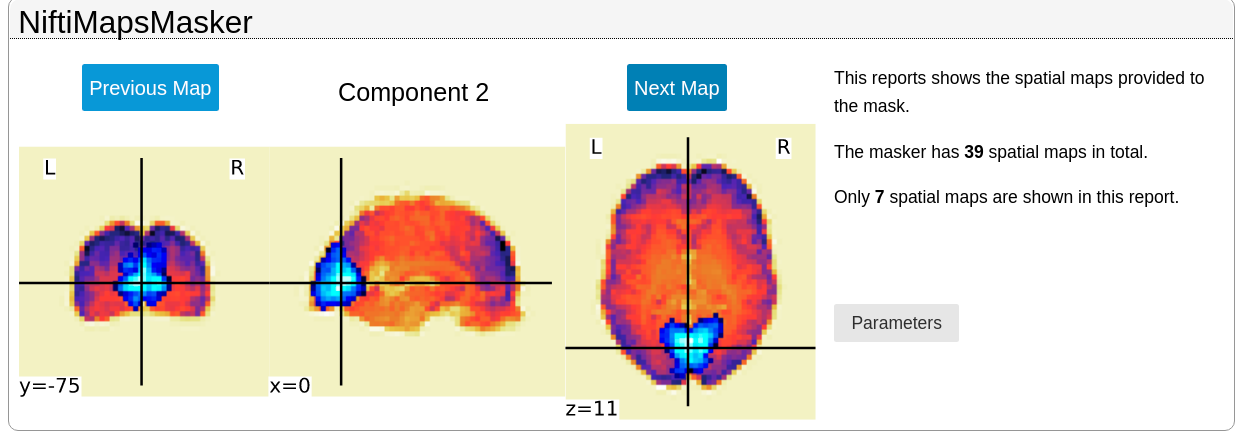
\includegraphics[scale=.8]{./figure_2}
	\caption{Example of surface based first level analysis.}
	\label{fig:figure_2}
\end{figure}

\newpage

\bibliographystyle{plain} 
\bibliography{bibliography}

\end{document}